\documentclass[11pt]{examdesign}
\usepackage{ucs}
\usepackage[T2A]{fontenc}
\usepackage[utf8]{inputenc}
\usepackage{amsmath}
\usepackage{pifont}
\usepackage{graphicx}
\usepackage{verbatim}
\usepackage[ddmmyyyy]{datetime}
\renewcommand{\dateseparator}{.}
%\SectionFont{\large\sffamily}
\usepackage[margin=1.5cm]{geometry}
\IncludeFromFile{sp_pa_test_code.tex}
%\Fullpages
\ContinuousNumbering
%\ShortKey
\DefineAnswerWrapper{}{}

%\NumberOfVersions{1}

\def\namedata{Name: \hrulefill \\[5pt]
ID: \hrulefill}

\begin{examtop}
{\parbox{.5\textwidth}{\textbf{\classdata} \\
\examtype, 30.09.2014\\ \emph{Each question
has exactly \textbf{one correct} answer.}}
\hfill
\parbox{.45\textwidth}{\normalsize \namedata}}
\end{examtop}

\def\aftersectsep{0pt}
\def\beforesectsep{0pt}
\def\beforeinstsep{0pt}
\def\afterinstsep{0pt}


\class{\Large{Structured Programming}}
\examname{Pre Programming Test}
\begin{document}
%\SectionPrefix{Дел \arabic{sectionindex}. \space}


\begin{multiplechoice}[title={Programming Apptitude},suppressprefix=no,rearrange=no]
\begin{question}
Which of the following is least like the others?
    \choice{cube}
    \choice{sphere}
    \choice{pyramid}
    \choice[!]{circle}
\end{question}

\begin{question}
Consider a language which uses the following set of characters:

Small set: { a b c }\\
Large set: { A B C }

Punctuation set: { x y }

This language must follow the following rules:
\begin{enumerate}
  \item A punctuation character must end all series. 
  \item A series can have up to but no more than 4 characters, including punctuation characters. 
\end{enumerate}    

Does the following series follow all the rules of the language defined above?

axBy
    
    \choice[!]{YES}
    \choice{NO}
\end{question}

\begin{question}
Consider the following flow chart for a customer:
\begin{center}
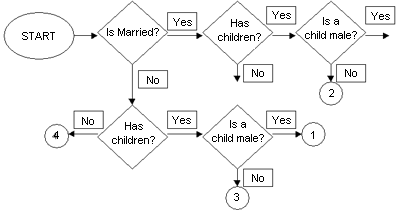
\includegraphics[scale=0.7]{apt}
\end{center}
The person in No.1 is:
  \choice{Married, with children}
  \choice{Married, with at least one son}
  \choice{Unmarried, with at least one daughter}
  \choice[!]{Unmarried, with at least one son}
  \choice{Unmarried, with no children}
\end{question}

\begin{question} 

Susan can type 10 pages in 5 minutes. Mary can type 5 pages
in 10 minutes. Working together, how many pages can they type in 30 minutes?

    \choice{15}
    \choice{20}
    \choice{25}
    \choice{65}
    \choice[!]{75}
\end{question}

\begin{question}
Consider the following series:

3, 4, 6, 9, 13, \underline{\hspace*{1cm}} What comes next?

    \choice{15}
    \choice{16}
    \choice{17}
    \choice[!]{18}
    \choice{19}
\end{question}

\end{multiplechoice}


\begin{shortanswer}[title={Define in a sentence (or two) the following terms?},
rearrange=no]

\begin{question}
Compiler?
\examvspace*{2cm}
\begin{answer}
The answer
\end{answer}
\end{question}

\begin{question}
Syntax error?
\examvspace*{2cm}
\end{question}


\begin{question}
Variable?
\examvspace*{2cm}
\end{question}

\begin{question}
I/O?
\examvspace*{2cm}
\end{question}

\begin{question}
CPU?
\examvspace*{2cm}
\end{question}

\end{shortanswer}

\end{document}
